\section{旁轴波动方程}
标量波动方程不像傅里叶(Fourier)方程,是允许密度与速度有任意的空间变动的。
你也许因为这一点而期望能把它直接用于偏移剖面的生产,但其实它很少用于偏移,因而我
们将首先回顾一下为什么会这样,然后我们将会讨论旁轴波动方程(paraxial wave equation),
它是大多数生产性偏移处理的基础。

就基本原理而言,旁轴波动方程可以说是射线和平面波这类简单概念与波动方稈湿体现
深刻概念之间的一釉折衷产物。旁轴波动方程也称作单平方根方程(Single-square-root
equation),在第二章中,它有一个专用名词,称作抛物线波动方程(parabolic wave
equation)导出抛物线波动方程不是从古典物理的简单概念着手的,它的建立就像量子物理
学中的薛丁格方程(Schroedinger equation)那样,颇为转弯抹角,
你必须下点功夫研究,才看得出为什么需要如此。当我在1970年把抛物线波动方程引进到
地震计算中去时,曾经遇到相当多的怀疑。你很幸运,多年的经验已经使我能比较好地完成
解释它的任务了。对我来说,也很幸运,这种方法在工业应用舞台上占有优势地位将会引起
你坚持学下去的兴趣。

旁轴波动方程将藉助于傅氏变换方法导出。傅氏变换方法同空间可变系数是不相容的,
由于我们想使速度体现出空间变化,需要最大限度地避免这种限制性,所以在傅氏变换域内
得到旁轴方程之后,就将$ik_x$用$\partial /\partial x$代替,将认$ik_z$用
$\partial /\partial z$代替。由于现在是在空间域内了,速度
也可以是空间可变的了。所得结果是一种恒可用有限差分方法求解的偏微分方程。这种处理
办法已证明是成立的,但是学习偏移方法的新学生对这种处理还有疑虑,这是可以理解的。
考虑到这点,本节最后部分将讨论一种不采用傅氏变换方法而导出旁轴波动方程的办法。

\subsection{为何标量波动方程很少用于偏移}
要是偏移真能用标量波动方程处理而不是用旁轴方程,那事情就能简单一些了。确实,
偏移是可以甩标量波动方程处理,而且还有若干潜在的好处(Kosloff与Baysal,1983)。
但是,99\%以上的现行工业性偏移应用却是藉助旁轴方程完成的。

采用标量波动方程时的主要问题在于它会产生不希望有的层内多次反射,但是爆炸反射
面概念却是不能处理多次波的。一次反射只能用上行波模拟,而多次反射既涉及上行路程又涉
及下行路程,实际工作中观察到的多次反射完全不同于爆炸反射面概念预言的结杲。对海底
多次反射来说,双程旅行时间深度为$t_0$的海底在$2t_0$、$3t_0$、$4t_0\ldots\ldots$等时刻形成海底多次反
射;在基于爆炸反射面概念的模型中,单程旅行时间深度为的海底是在$3t_0$、$5t_0$、$7t_0\ldots\ldots$
等时刻形成海底多次反射。在制造望远镜、显微镜或摄影机时,设计者很注意要压制向后反
射的光,因为它在影像上形成背景干扰。与此类似,在建立一个偏移程序时,我们不希望有
对聚焦成像毫无作用的能量在周围移动。带有空间可变系数的标量波动方程就会产生此类能
量,如果它是相干能量而且偏移至一次波较弱的某个时间上,这种不受欢迎的能量就特别麻
烦。它之使人烦恼讨厌,正如在电视屏幕上能见到明亮窗户的反射影子一样令人烦恼。所
以,你如果要试图用标量波动方程来进行偏移,你就得使速度尽可能地平滑。

采用标量波动方程进行成像时的另一种困难是由于倏逝波所形成的,这些波是随深度而
指数增长或衰变的波。大自然是沿正向时间将波外推,而我们则将它们向深度方向外推。增
长指数有微不足道的扰动、甚至数值上是可舍入的零头,就能产生很大影响。因为它增长速
度快,所以必须找到某些手段来压制它们。

采用标量波动方程进行成像时的第三个困难源出于初始条悴。标量波动方程有一项深
度$z$的二阶导数,这意味着要求在$z$轴上有两个边界条件。因为数据是在$z=0$时记录的,看来
很自然,这些边界条件就应该是$z=0$时的波场$P$和波场梯度$\partial P/\partial z$、,可是$\partial P/\partial z$如并没有在地面上记录。

幸好,建立某神整个是在计算机内部运算的成像方法时,我们有理想的工具可资利用,
这就是无反射透镜。或者说,我们不是用现实世界的标量波动方程而是用旁轴波动方程。

\subsection{旁轴波动方程的Fourier导出方法}
现在从标量波动方程的波散关系开始
\begin{equation}
k_x^2+k_z^2=\frac{\omega^2}{v^2}
\label{eq:ex1.5.1}
\end{equation}
取平方根
\begin{equation}
k_z=\pm\sqrt{\frac{\omega^2}{v^2}-k_x^2}
\label{eq:ex1.5.2}
\end{equation}
在式\ref{eq:ex1.5.2}内选择负号,意味着是取上行波而消去下行波。式\ref{eq:ex1.5.1}是标量波动方程\\
$\frac{\partial^2 P}{\partial x^2}+\frac{\partial^2 P}{\partial z^2}=\frac{1}{v}\frac{\partial^2 P}{\partial t^2}$\\
的三维傅氏变换结果,对式\ref{eq:ex1.5.2}进行反变换则将给出一个仅为上行波(或下行波)而
无其他波的方程。对某个坐标轴的逆傅氏变换只不过是选择下列一种代换的问题
\begin{subequations}\label{eq:ex1.5.3}
\begin{equation}
\frac{\partial}{\partial t}=-i\omega
\end{equation}
\begin{equation}
\frac{\partial}{\partial x}=ik_x
\end{equation}
\begin{equation}
\frac{\partial}{\partial z}=ik_z
\end{equation}
\end{subequations}
对$z$轴进行逆变换之后,就得一个关于$z$的偏微分友程。速度在该方程中可以取$z$为变量,对
$x$轴也可得类似结果。式\ref{eq:ex1.5.3}中任何一种代换代入式\ref{eq:ex1.5.2}而得出的任何一种结果,就
称为旁轴方程,本书第二章将详细讨论这些方程的意义。在开始这样解释旁轴波动方程之前,
要讨论一下不采用傅氏变换如何导出它。除了获得导致基本偏移方程的清晰思路之外,这种
导出方法还能使我们更好地理解该方程真正能作什么,以及它如何不同于标量波动方程。
\subsection{斯涅尔(Snell)波}
研究波扬很自然要从描述恒速介质内的平面波的方程开始。不过,在反射地震勘探中,
最浅与最深反射面之间的速度差异一般都超过两倍,为此,在分析野外资料时差不多总得包括
速度随深度的变化。除了要迁就适应分层速度$v(z)$)以外,地震学理论需要考虑的正是像乎
面波那样的波。图\ref{fig:omk/airplane}所示就是这样一种理想情形:水平飞行的超音速飞机辐射出的波传
播进入地下。
\begin{figure}[H]
\centering
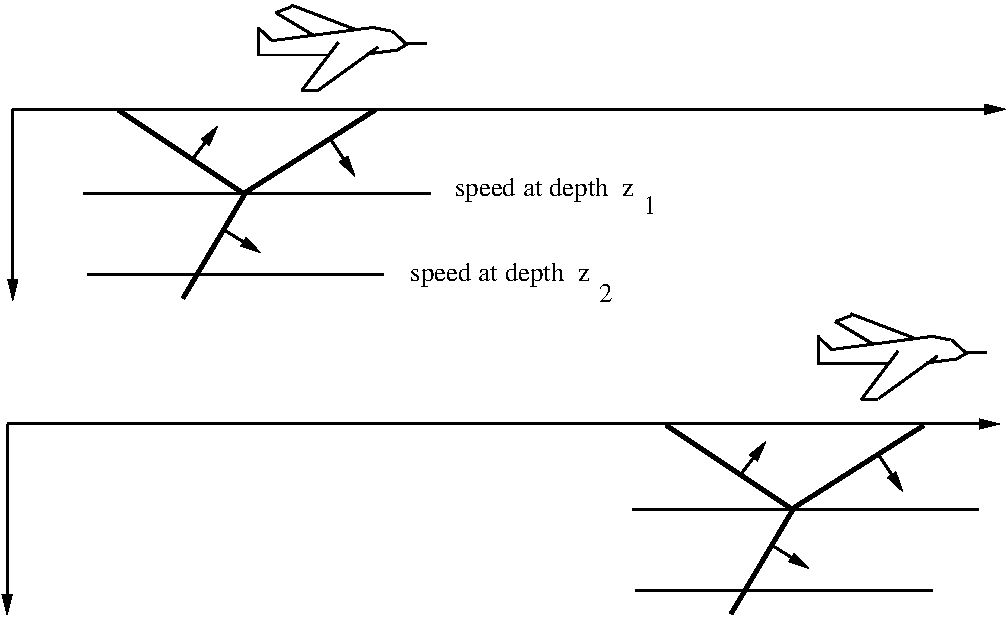
\includegraphics[width=0.5\textwidth]{omk/airplane}
\caption[airplane]{疾翔的飞机辐射出声波进入地中。由图你可得出结论:在深度为$z_1$之处和深度为$z_2$之处的
$\partial t/\partial x$是相同的;在各向同性介质中,这个结论就导出Snell定律}
\label{fig:omk/airplane}
\end{figure}
飞机以恒速水平飞行,从$x=-\infty$飞至$x=+\infty$。试想像有一水平平面成层地层,在这种模
型中,尤轴上的任何点同$x$轴上任何其他点之间毫无区别,但是地震波速度是逐层变化。可能
存在反射、折射、横波及多次反射。不管图形如何,它是随飞机而一起运动的,于是可想像
飞机附近的波阵面图像也随飞机而一起运动。即使地层速度是随深度而增大的,该图的顶部
与图的底部也都是以相同速度沿
水平方向运动,如果顶部与底部不是相同速度,图形就会畸变,
同所假设的平移对称性相矛盾。这种水平速度,或更确切地说,这
种速度的倒数$\partial t/\partial x$,有若干个名称,在实际工作中,将它称作时
差。在理论工作中,则称它为射线参量。注意到这点是非常重要
的:$\partial t/\partial x$不随深度而变化,即便地震波速度是随深度而变化
的。在恒速介质中,波传播方向的角度不随深度而变化,在成层
介质中,$\partial t/\partial x$不随深度而变化。

波的微分几何关系如图\ref{fig:omk/frontz}所示。该图表明
\begin{subequations}\label{eq:ex1.5.4}
\begin{equation}
\frac{\partial t}{\partial x}=\frac{sin\theta}{v}
\label{eq:ex1.5.4a}
\end{equation}
\begin{equation}
\frac{\partial t}{\partial z}=\frac{cos\theta}{v}
\label{eq:ex1.5.4b}
\end{equation}
\end{subequations}

这两个方程定义两个速度(速度倒数)。第一个是沿地表面测定的
水乎速度,称为水平相速度;第二个是沿钻孔深度方向测定的垂
直速度,称为垂直相速度。注意,这些速度全都大于波在介质
中的传播速度$v$。由波阵面在坐标轴上的投影得出的速度都大于
$v$,而由射线在坐标轴上的投影得出的速度都小于$v$。相速度的倒数称为时差(stepout
)或者慢度(slowness)。
\begin{figure}[H]
\centering
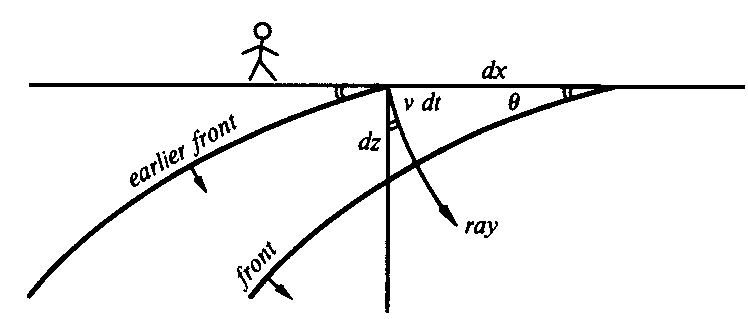
\includegraphics[width=0.5\textwidth]{omk/frontz}
\caption[frontz]{成层介质$v(z)$中的下行波阵面与射线,波阵面彼此平行平移}
\label{fig:omk/frontz}
\end{figure}

斯涅尔定律将波在一层内的传播角度同在另一层内的传播角度联系在一起。式\ref{eq:ex1.5.4a}
沿深度方向应恒定不变,实际上正是斯涅尔定理的证明。确实,我们已经导出的正是斯涅尔
卑律在地震学中,所有的波均在速度分层介质中传播,所以不能把它们称为平面波。但是
我们需要对接近于平面波的那些波取个名宇,将平面波概念推广至成层介质$v(z)$的情形,把它
定义为斯涅尔波。一个平面波恰好进入速度$v(z)$随深度而变的某种介质,就变成了一个斯涅
尔波,当平面波具有某种传播方向角度时,就用一个斯涅尔参量$p=\partial t/\partial x$来代替斯涅尔波。

值得注意的是,斯涅尔参量$p=\partial t/\partial x$加可在地面上直接观测,而$v$与$\theta$却没一个能直接观
测。因为$p=\partial t/\partial x$不但可观测,而且沿深度方向恒定不变,所以习惯上都利用这点从式\ref{eq:ex1.5.4a}
中消去$\theta$
\begin{subequations}\label{eq:ex1.5.5}
\begin{equation}
\frac{\partial t}{\partial x}=\frac{sin\theta}{v}=p
\label{eq:ex1.5.5a}
\end{equation}
\begin{equation}
\frac{\partial t}{\partial z}=\frac{cos\theta}{v}=[\frac{1}{(v(z))^2}-p^2]^{1/2}
\label{eq:ex1.5.5b}
\end{equation}
\end{subequations}
令斯涅尔波通过零时间的原点,则任何其他位置上的斯涅尔波到达时间表达式由下式给
出
\begin{subequations}\label{eq:ex1.5.6}
\begin{equation}
t(x,z)=\frac{sin\theta}{v}x+\int_0^x\frac{cos\theta}{v}dz
\label{eq:ex1.5.6a}
\end{equation}
\begin{equation}
t(x,z)=px+\int_0^x[\frac{1}{(v(z))^2}-p^2]^{1/2}dz
\label{eq:ex1.5.6b}
\end{equation}
\end{subequations}
计算出$\partial t/\partial x$与$\partial t/\partial z$,然后与式\ref{eq:ex1.5.5}比较,很容易检查证明式
\ref{eq:ex1.5.6b}成立。

斯涅尔波可具有任意波形$f(t)$,利用式\ref{eq:ex1.5.6}定义一个延迟时间$t_0$,则位于$(x,z)$
位置上的延迟波$f[t-t_0(x,z)]$将为
\begin{equation}
SnellWave(t,x,z)=f[t-px-\int_0^x[\frac{1}{(v(z))^2}-p^2]^{1/2}dz]
\label{eq:ex1.5.7}
\end{equation}
\subsection{时移方程}
在已知地面上的波形条件下,预测地层内部的波场,是一项重要任务。对于下行平面
波,可用下列时移偏微分方程实现这点
\begin{equation}
\frac{\partial P}{\partial z}=-\frac{1}{v}\frac{\partial P}{\partial t}
\label{eq:ex1.5.8}
\end{equation}
将试验解
\begin{equation}
P=f(t-\frac{z}{v})  \quad\quad\quad for\quad constant\quad v
\label{eq:ex1.5.9}
\end{equation}
或
\begin{equation}
P=f(t-\int_0^z\frac{dz}{v(z)})  \quad for\quad v(z)
\label{eq:ex1.5.10}
\end{equation}
代入很容易就能证明确实如此。

对于非垂直入射情形,下述偏微分方程也能成立
\begin{equation}
\frac{\partial P}{\partial z}=-\frac{\partial t}{\partial z}\frac{\partial P}{\partial t}
\label{eq:ex1.5.11}
\end{equation}
该方程的解为
\begin{equation}
P=f(t-px-\int_0^z\frac{\partial t}{\partial z}dz) 
\label{eq:ex1.5.12}
\end{equation}
解释式\ref{eq:ex1.5.11}与\ref{eq:ex1.5.12}时,要记住$1/(\partial t/\partial z)$是垂向视速度。波场$P$关于深度$z$的偏
导数是在恒定$x$时取的,即向下外推波场。只用时移就可达到向下外推效果的这种思想,仅
当存在一个斯涅尔波时才成立,就是说,在所有位置上看见的必须是同一个任意时间函数。

将式\ref{eq:ex1.5.5}代入时,还能使我们把式\ref{eq:ex1.5.11}改写成各种不同的形式
\begin{subequations}\label{eq:ex1.5.13}
\begin{equation}
\frac{\partial P}{\partial z}=-\frac{cos\theta}{v}\frac{\partial P}{\partial t}
\label{eq:ex1.5.13a}
\end{equation}
\begin{equation}
\frac{\partial P}{\partial z}=-[\frac{1}{(v(z))^2}-P^2]^{1/2}\frac{\partial P}{\partial t}
\label{eq:ex1.5.13b}
\end{equation}
\begin{equation}
\frac{\partial P}{\partial z}=-[\frac{1}{(v(z))^2}-(\frac{\partial t}{\partial x})^2]^{1/2}\frac{\partial P}{\partial t}
\label{eq:ex1.5.13c}
\end{equation}
\end{subequations}
式\ref{eq:ex1.5.13}是一个旁轴波动方程。由于$\partial t/\partial x=p$可沿地表面测定,看来将方程\ref{eq:ex1.5.13c}同某 种观测数据$P(t,x,z=0)$和假设的一种速度$v(z)$结合一起,将使我们有可能确定。这是
向下延拓的必要的第一步,不过必须假设仅存在一个斯涅尔波而不是若干斯涅尔波的叠加才
行。不同斯涅尔路程上的不同波形叠加起来,就会造成在不同位置上看到不同时间函数的结
果。于是,仅一次时移将达不到向下延拓的目的。幸好,一个逐点可变的复杂波场能够分解
成许多斯涅尔波,其中每一个均可用微分方程\ref{eq:ex1.5.13}或者它的解\ref{eq:ex1.5.12}来实现向下
延拓,这样一种分解方法就是傅里叶分析。 

\subsection{傅氏分解}
对地表面上看到的函数$f(x,t,z = 0)$进行傅里叶分析时,要求傅氏积分核为$exp(-i\omega t+ik_xx)$。以速度倒数
$\partial t/\partial x=k_x/\omega$沿地表面运动时,傅氏积分核的相位应保持为常数,因而
也就是积分核本身保持为常数。这时,只有以与斯涅尔波相同的速度运动的那些正弦分量,
才可以使该斯涅尔波具有非零的相关关系。因此,如果扰动是一个斯涅尔波,则除了满足
$p=k_x/\omega$关系的那些分量之外,所有傅氏分量均为零。你应当记住这些基本关系
\begin{equation}
\frac{\partial t}{\partial x}=\frac{sin\theta}{v}=p=\frac{k_x}{\omega}
\label{eq:ex1.5.14}
\end{equation}
在理论地震学中,由于利用式\ref{eq:ex1.5.14}求取一个余弦,结果总是出现平方根函数。

利用斯涅尔参量户的这种傅氏变换域解释,能使我们把平方根方程\ref{eq:ex1.5.13}写成更为
有用的形式。但是首先必须在傅氏变换域内表达平方根方程,将\ref{eq:ex1.5.13}中的算子$\partial /\partial t$用
$-i\omega$代替,就可完成这点,结果为
\begin{equation}
\frac{\partial P}{\partial z}=+i\omega[\frac{1}{(v(z))^2}-\frac{k_x^2}{\omega^2}]^{1/2}P(\omega,k_x,z)
\label{eq:ex1.5.15}
\end{equation}
现在,它等价于把微分方程\ref{eq:ex1.5.15}
或者它的解\ref{eq:ex1.5.12}具体化为如下复指数,
\begin{equation}
P(\omega,k_x,z)e=exp\{i\omega\int_0^z(\frac{1}{(v(z))^2}-\frac{k_x^2}{\omega^2})^{1/2}dz\}
\label{eq:ex1.5.16}
\end{equation}
以后,当我们考虑可横向变化的速度$v(x)$时,这个解\ref{eq:ex1.5.16}就变成错误的了,然而微分方程\ref{eq:ex1.5.13c}描述任何局部平面波性态却仍旧有效。但是,在准备处理横向速度梯度问题
以前,我们应当更仔细地研究一下垂直速度梯度。

\subsection{速度梯度}
将斯涅尔波场表达式代入标量波动方程中时,我们发现,我们的斯涅尔波的定义并不满
足该标量波动方程。不过,这种偏差仅发生在出现有速度梯度时。换言之,如果浅层恒定速度
为$v_1$,深层恒定速度为$v_2$,则除了在$v_1$变为$v_2$之处外,方程处处可被满足。因透过系数之
故,经过分界面时,标量波动方程的解必然表现有振幅变化,我们所定义的斯涅尔波则是一
种随深度之变化而只有恒定振幅的波。旁轴波动方程可加以修正,使之能反映透过系数的影
响。现在所以很少进行这种修正,其原因可能同恒可忽略密度梯度的原因相同,在它们可改
善所得结果、即给出更正确的振幅与可能的微小相移的同时,它们也使方程增加了杂乱干扰
的影响,抵销了所得好处。说实在的,如果要求这样作,那么就应当回答其他更深刻的问
题,诸如为什么不是利用标量弹性方程的各种不同其他形式而是利用声学方程。

即使修正旁轴波动方程使之能同透过系数影响结合起来,但由于缺乏反射波,它的解将
仍然无法满足标量波动方程。但是那好极了,因为正是具有无反射透镜作用的旁轴方程才是
数据处理所期望的方程。

\subsection{习 题}
\begin{enumerate}
\item 试设计一种平面波数学表达式,要求它是时间的脉冲函数,传播方向与垂直轴2正
方向所夹角度为15°。试在下列域内表示所得结果
\begin{table}[!ht]
\centering
\ttfamily
\small
%\begin{tabularx}{\textwidth}{Y|Y}
\begin{tabular}{p{3cm}p{4cm}}
\toprule
\midrule
 (a)& $(t,x,z)$\\
 (b)&$(\omega,x,z)$ \\
 (c)&$(\omega,k_x,z)$\\
 (d)&$(\omega,p,z)$ 
%\bottomrule
%\end{tabularx}
\end{tabular}
\end{table}
\item 试求振幅函数$A(z)$,当乘以式\ref{eq:ex1.5.12}中的函数$f$时,可成为分层介质$v(z)$的
标量波动方程近似解。对于$p=0$的情形,该解应化简为1.4节中习题(2)的解。
\end{enumerate}

